\chapter{Cifrari Storici}

I cifrari storici sono tutti quei cifrari ideati prima degli anni 70. Questi sono quasi del tutto insicuri al giorno d'oggi. Prima di andare ad analizzare questi primi cifrari, diamo alcune definizioni utili:
\begin{itemize}
    \item \textbf{Spazio delle chiavi K}: spazio contenente tutte le possibili chiavi del sistema crittografico;
    \item \textbf{Spazio dei messaggi M}: insieme di tutti i messaggi (o simboli) che si possono cifrare;
    \item \textbf{Spazio dei crittotesti C}: insieme di tutti i possibili crittotesti generabili dal sistema di cifratura;
    \item \textbf{Keygen}: funzione di generazione delle chiavi;
    \item \textbf{Encryption, Enc(k,m) o $Enc_k$}: funzione che permette la cifratura del messaggio;
    \item \textbf{Decryption, Dec(k,c)}: funzione che permette la de cifratura di un crittotesto. 
\end{itemize}

\section{Shift Cipher}
Il primo cifrario storico che analizzeremo è il cifrario per \textbf{Shift}. Per cui, avremo lo spazio delle chiavi K con 25 elementi e, per generare una chiave, ne decidiamo una a caso.\footnote{Definiamo come \textbf{cifrario di Cesare}, il cifrario Shift con chiave uguale a 3.} Dopodiché, associamo ad ogni lettera dell'alfabeto un numero (ad esempio $A=0, B=1, ecc...$) ed effettuiamo una \textit{somma circolare}\footnote{Somma per cui, una volta arrivati al massimo si riparte da 0.} tra il numero associato e la chiave. Fatto ciò, riportiamo i numeri nelle lettere corrispondenti e avremo ottenuto il crittotesto. Per decifrarlo procederemo semplicemente al contrario. 

Notiamo a primo impatto come questo cifrario non sia sicuro poiché, anche andando per tentativi, si arriva facilmente a decifrare il testo poiché il numero di chiavi possibili è molto limitato. Capiamo subito quindi che un buon cifrario deve avere uno spazio delle chiavi grande abbastanza da non permettere di provare tutte le chiavi a casaccio. 

\section{Cifrario per sostituzione}
L'idea alla base rimane quella di sostituire le lettere con altre. Cambiamo semplicemente lo spazio delle chiavi per cui ogni $k \in K$ sarà adesso una permutazione dei simboli $0,1,2,...,25$ e per cifrare un simbolo, lo sostituiremo con il simbolo corrispondente nella chiave. Se $A\xleftarrow{}K, C\xleftarrow{}T, S\xleftarrow{}D$, avremo che $CASA = TKDK$.
Adesso la situazione cambia, il numero di chiavi possibili è molto alto e, considerando tutti i possibili caratteri ASCII, avremo un alfabeto di 256 caratteri, per cui avremo $256!$ chiavi che è circa $2^{896}$ e, anche considerando di poter elaborare $10^{12}$ chiavi al secondo, ci vorrebbero circa 14 miliardi di anni per trovare la chiave corretta.

Tuttavia, nonostante questo sembri rassicurarci, possiamo, tramite una semplice ricerca su internet, conoscere le statistiche che riguardano la presenza delle varie parole nelle parole della lingua italiana. 
\begin{figure}[H]
    \centering
    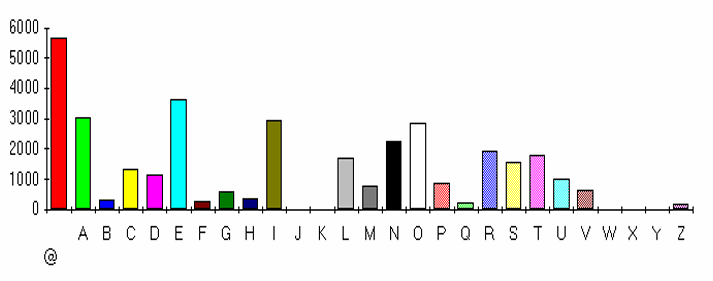
\includegraphics[width=0.5\linewidth]{Images/promessi_sposi.png}
    \caption{Frequenza delle varie lettere nel primo capitolo dei promessi sposi.}
\end{figure}

Grazie a queste informazioni, ci basta semplicemente andare a sostituire, in base alle frequenze trovate nel testo, le lettere con maggiore riscontro e, piano piano, con un testo sufficientemente grande, riusciremo a decifrare il testo. 
\section{One Time Pad e Sicurezza Perfetta}
Sia SE\footnote{Cifratura simmetrica.} = (Keygen, Enc, Dec), diremo che è \textbf{Perfettamente sicuro} se
\[\forall m1,m2\in M\quad \forall c \in C\quad Pr[Enc(k,m_1)=c] = Pr[Enc(k,m_2)=c]\] \footnote{In questa definizione k è variabile.}

Definiamo One Time Pad come:
\begin{itemize}
    \item $K=M=C=\{0,1\}^l$ questo schema ci indica che lo spazio delle stringhe è composto da \{0,1\} di lunghezza $l$;
    \item KeyGen(l) = $K \xleftarrow{random}\{0,1\}^l$ generiamo una chiave lunga l composta solo da 0 e 1;
    \item Enc(K,M) = $K \oplus M = C$; 
    \item Dec(K,M) = $K\oplus C = M$
\end{itemize}
Questo cifrario è \textit{perfettamente sicuro} se la chiave viene utilizzata solo una volta. Possiamo dimostrare ciò verificando la condizione citata prima.
Dati $m_1,m_2$ e $c$:
\[Pr[Enc_k(m_1)=c] = Pr_k[k\oplus m_1 =c] = Pr_k[k = m_1 \oplus c] = 1/2^l\]
\[Pr[Enc_k(m_2)=c] = Pr_k[k\oplus m_2 =c] = Pr_k[k = m_2 \oplus c] = 1/2^l\]
\\
E $1/2^l$ corrisponde esattamente alla probabilità che k sia esattamente quella. Possiamo ancora testare questa proprietà per dimostrare che il cifrario per sostituzione non sia perfettamente sicuro. Per fare ciò, ci basta verificare che la proprietà non sia soddisfatta anche solo per una coppia da noi arbitrariamente scelta. 
Scegliamo $m_1 = \text{ciao} \quad m_2=\text{dado} \quad c=\text{abcd}$ e su queste calcoliamo le probabilità.
\begin{align*}
    &Pr[Enc_k (m_1)=c] = Pr_k[Enc_k(ciao)= abcd] = \frac{22!}{26!}\\
    &Pr[Enc_k (m_2)=c] = Pr_k[Enc_k (dado)=abcd] = 0
\end{align*}

Come possiamo vedere, la probabilità che $m_2$ sia cifrato in abcd è 0 poiché non è possibile raggiungere questa configurazione dato che ad una lettera se ne può associare solo un'altra e dado ha due lettere uguali.
Possiamo anche dimostrare che One Time Pad è perfettamente sicuro solo se utilizziamo la chiave una sola volta. Nel caso di riutilizzo della chiave, un messaggio sarà una stringa $(x||y)^{\{0,1\}^{2l}} \oplus (k||k)^{\{0,1\}^{l}}$. Testando la proprietà:
\begin{align*}
    &m_1=0^{2l} \quad m_2 = 0^l||1^l\\
    &Pr[Enc_k(m_1)=c] = 1/2^l \quad Pr[Enc_k(m_2)=c] =0
\end{align*}

Un ultimo test lo possiamo effettuare verificando cosa succederebbe se togliessimo la chiave composta da una serie di 0 su One Time Pad. A primo impatto ci sembra una scelta sicura poiché non rischiamo che il messaggio passi in chiaro. Verifichiamo la proprietà:
\begin{align*}
    &m_1!=m_2 \quad c=m_2\\
    &Pr[Enc_k(k,m_1)=c] = Pr_k[k\oplus m_1 = c] = Pr_k[k = m_1 \oplus c] = \frac{1}{2^l-1}\\
    &Pr[Enc_k(k,m_2)=c] = Pr_k[k\oplus m_1 = c] = Pr_k[k = m_2 \oplus c] = 0
\end{align*}

Dimostriamo che questo sistema, contro intuitivamente, non è perfettamente sicuro. Il punto è che, anche se il messaggio passasse realmente in chiaro, l'avversario non avrebbe modo di stabilirlo e, dunque, non gli sarebbe utile. 

\section{Limitazioni della Perfetta Sicurezza}
Sia (KeyGen, Enc, Dec) uno schema perfettamente sicuro, M uno spazio dei messaggi e K lo spazio delle chiavi, allora $|K| \ge |M|$.

Supponiamo per assurdo che $|M| > |K|$ e che $c\in C$ sia un crittotesto raggiungibile almeno tramite una chiave. 
\[M(c) = \{m:Dec_k(c)=m\}\]
Sappiamo che:
\[1\leq |M(c)| \leq |K| \leq |M|\]
Per cui, prendiamo $m_2\in M ,\quad m_2\notin M(c)$ e $m_1\in M(c)$. Avremo che: 
\begin{align*}
    &Pr[Enc_k(m_1)=c] \neq0\\
    &Pr[Enc_k(m_2)=c]  = 0
\end{align*}
\section{Teorema di Shannon}
SE = (KeyGen, Enc, Dec), $|M|=|K|=|C|$, SE offre perfetta sicurezza se e soltanto se:
\begin{enumerate}
    \item $\forall k \in K$, K è scelta con probabilità 1/$|K|$;
    \item $\forall m \in M, \forall c\in C, \exists! k\in K$ tale che $Enc(k,m) = c$.
\end{enumerate}

\chapter{Cifratura a blocchi}
In crittografia un algoritmo di cifratura a blocchi è un algoritmo a chiave simmetrica operante su un gruppo di bit di lunghezza finita organizzati in un blocco. A differenza degli algoritmi a flusso che cifrano un singolo elemento alla volta, gli algoritmi a blocco cifrano un blocco di elementi contemporaneamente.

\[E: \{0,1\}^k * \{0,1\}^n \xrightarrow{} \{0,1\}^m\]
\\
E questa deve godere delle seguenti proprietà:
\begin{enumerate}
    \item Invertibile una volta fissata una chiave;
    \item Deve essere efficace e veloce;
    \item E deve essere "sicuro". 
\end{enumerate}

DES fu il primo cifrario a blocchi nato per scopi militari e questo, dovendo funzionare solo su specifici hardware, risultava parecchio performante per gli hardware su cui si basava ma le performance calavano quando dall'hardware si passava al software. Per DES la chiave k era composta da 56 bit mentre il blocco era composto da 64 bit.\footnote{Vedremo poi perché queste scelte sono problematiche.} A causa del fatto che questo algoritmo avesse basse performance dal punto di vista software, si decise di sostituirlo andando alla ricerca di un cifrario con dimensioni di chiave e blocchi maggiori e più veloci. 
Per fare ciò venne indetto un concorso pubblico e, tra tutti gli algoritmi di cifratura proposti, la scelta ricadde sull'algoritmo Rijndael che poi divenne lo standard \textbf{AES}. 
\section{Advanced Encryption Standard}
Questo algoritmo di cifratura a chiave simmetrica fu quello che sostituì totalmente l'algoritmo DES e che fu' adottato pure dai servizi segreti americani per cifrare documenti top secret. 
AES si divide in tre livelli fondamentali detti \textbf{layers} e, ognuno di questi, manipola tutti i bit dello \textit{stato}.\footnote{Lo stato è un valore inizialmente inizializato a M e che come stato finale il crittotesto C.} Avremo:
\begin{itemize}
    \item \textbf{Key addition layer:} in cui lo stato attuale viene aggiornato usando una chiave di round di 128 bit. Questa chiave in realtà è composta da 11 sotto-chiavi che vedremo dopo nello specifico come vanno ad agire;
    \item \textbf{Byte Substitution layer:} lo stato è modificato da operazioni non lineari. È importante che non lo siano poiché altrimenti basterebbe risolvere un sistema lineare per rompere il cifrario;
    \item \textbf{Diffusion layer}: diffonde tramite trasformazioni lineari tutti i bit dello stato. Si basa su due procedure che non sono altro che scambio di righe e scambio di colonne;
\end{itemize}

\begin{figure}[H]
    \centering
    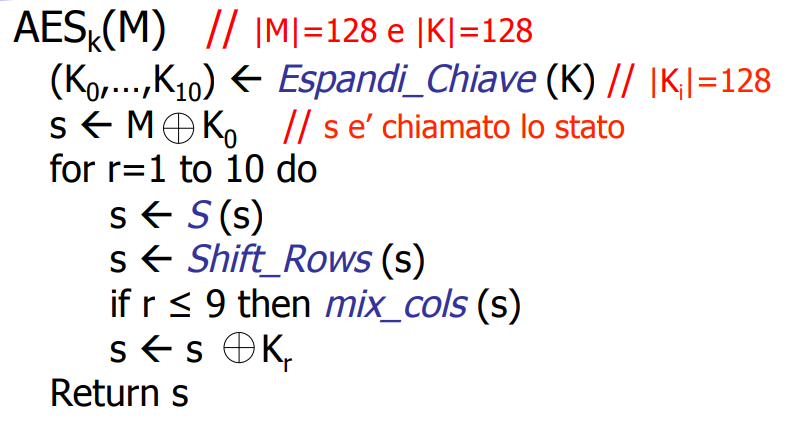
\includegraphics[width=0.5\linewidth]{Images/aes_algoritmo.png}
    \caption{Pseudo-codice dell'algoritmo AES.}
    \label{fig:algoritmo AES}
\end{figure}

La prima funzione che salta all'occhio è quella di \textbf{espansione} che non fa altro che prendere in input la chiave $K$ di 128 bit per poi produrre 11 sotto chiavi di 128 bit ciascuna. Prima di andare a vedere la procedura S, è bene dare alcune definizioni utili.

Sappiamo che possiamo rappresentare 1 byte come un generico polinomio di questo tipo $a_7x^7+a_6x^6+...+a_1x+a_0$. Per poter lavorare concretamente con questo polinomio, abbiamo bisogno di due operazioni che rispettino alcune proprietà:
\begin{enumerate}
    \item Vogliamo che la somma sia chiusa, per cui se facciamo una somma, il risultato non esce dall'insieme di riferimento;
    \item Vogliamo che valgano le proprietà \textbf{commutative} e \textbf{associativa};
    \item Vogliamo l'esistenza di un elemento neutro;\footnote{Se viene eseguita un'operazione tra un elemento e il neutro, l'elemento rimane invariato.}
    \item Ogni elemento deve avere un inverso; \footnote{Se viene eseguita un'operazione tra un elemento e il suo inverso, il risultato sarà l'elemento neutro.}
\end{enumerate}
Quando esistono due operazioni di questo tipo, allora parleremo di un \textbf{campo}. Nel nostro caso, avremo come operazioni:
\begin{itemize}
    \item \textbf{$\oplus$ XOR}: somma classica tra polinomi ma il tutto viene fatto modulo 2. Non a caso, per implementarlo viene utilizzato uno xor vero e proprio che è un'operazione estremamente efficiente in termini di calcolo. Esempio: 
    \[x^7+x^6+x^4+x+1 \oplus x^6+x^5+x^4+x = x^7+x^5+1\]
    \item \textbf{$*$ moltiplicazione:} facciamo la tipica moltiplicazione tra polinomi e, nel caso in cui si andasse in un polinomio oltre il grado 7 che quindi non rientrerebbe in un byte, effettuiamo una riduzione con un polinomio di grado 8 che, per AES, è $x^8+x^4+x^3+x+1$. Esempio:
    \[(x^7+x^6+x^4+x+1) * (x^6+x^5+x^4+x = x^7+x^5+1) = x^{13}+x^9+x^5+x^4+x^2+x\]
    Come già detto questo non rientra in un byte, dunque, facendo una semplice divisione tra polinomi, otteniamo $x^6+x^3+x^2+1$. In AES le moltiplicazioni si fanno tendenzialmente per potenze di due per cui l'operazione di moltiplicazione non è altro che uno shift a sinistra che, nel caso in cui si ecceda con il grado del polinomio, basta effettuare l'operazione di riduzione. Tuttavia, potendo eccedere solo al grado 8, la riduzione consisterà semplicemente in uno xor con il polinomio riduttore di AES.
\end{itemize}

In base a quanto detto, vedremo che l'operazione S di AES non è altro che una sequenza, seppur lunga, di shift e xor che sono operazioni efficientissime da implementare. 

L'operazione S è composta da due operazioni principali:
\begin{itemize}
    \item \textbf{inv'(a):} un'operazione in grado di trovare l'inverso di a. Vedremo poi che esistono dei modi particolari per ottimizzare questo processo;
    \item \textbf{aff(a):} un'operazione non lineare che consiste sostanzialmente in una moltiplicazione riga per colonna e poi una somma;
    \begin{figure}[H]
        \centering
        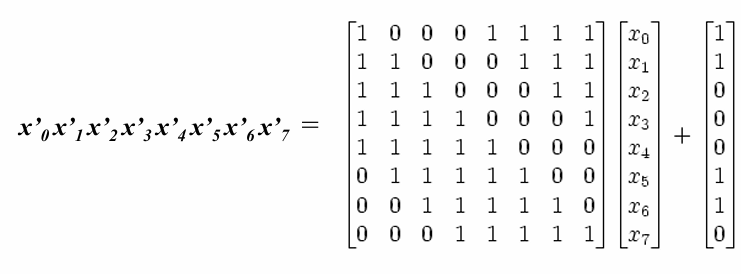
\includegraphics[width=0.8\linewidth]{Images/s_aff.png}
        \label{fig:operazione_affine}
    \end{figure}
\end{itemize}

Questo processo potrebbe ottimizzato ancora di più facendo alcune semplici considerazioni. Nel campo di Galois sono presenti alcuni elementi detti \textbf{generatori} che permettono, moltiplicandoli per sé stessi, di generare tutti i numeri del campo. Continuando con le potenze varrà sempre la proprietà $g^{255} = 1$ cioè l'elemento neutro della moltiplicazione da cui poi si ripartirà da capo se si continua.

Possiamo tabellare tutti i valori\footnote{La tabellazione di questi valori verrà fatta in momenti in cui il processore è libero, così da avere costo 0.} calcolati dalla potenza di un generatore memorizzando potenza-risultato e, sfruttando le proprietà delle potenze se $a=g^x$, allora $a^{-1} = g^{255-x}$. Così facendo, trasformiamo l'operazione d'inverso in una operazione di look-up sulla tabella.

Un'ulteriore ottimizzazione la si può ottenere tabellando in maniera diretta i risultati della funzione S box dato che questi sono costanti. Tuttavia, questa tabella può essere utilizzata solo se si ha la certezza che non potrà essere modificata quando in memoria, quindi bisogna stare attenti a quando implementare questa funzione.

Per quanto riguarda invece la funzione shift-rows e shift-cols, si tratta di disporre gli stati in una matrice\footnote{Dall'alto verso il basso} per poi effettuare degli scambi. Per quanto riguarda shift-rows la prima riga rimane invariata, la seconda fa uno shift a sinistra di una posizione, la terza shift di due posizioni a sinistra e così via. La mix-cols fa più o meno la stessa cosa. 

Quello che vogliamo adesso è trovare una proprietà di sicurezza che ci garantisce in maniera certa che il sistema è sicuro. Verifichiamo cosa succede se il sistema è sicuro rispetto a un \textbf{attacco di Key Recovery}. Immaginiamo di essere un attaccante e di poter vedere blocco di input e blocco di output e di poter mandare noi stessi i messaggi. Infine, analizzando questi, vogliamo trovare la chiave. AES è sicuro rispetto a questo tipo di attacco ma domandiamoci, è una condizione sufficiente a dire che il nostro sistema è sicuro?
Prendiamo un cifrario $E_k(x) = x$, questo è sicuro da attacchi di key recovery dato che, banalmente, la chiave non la stiamo utilizzando. Capiamo quindi che questa proprietà è sì necessaria, ma non è sufficiente a dire che il nostro sistema è sicuro.
Proviamo adesso a verificare se il sistema è sicuro rispetto ad \textbf{attacchi di Plain-Text Recovery.} In questo scenario l'attaccante avrà a disposizione esclusivamente i messaggi cifrati e cercherà di decifrarli non necessariamente estraendo la chiave. Anche in questo caso, AES è sicuro da questo tipo di attacchi, tuttavia anche questa è una condizione necessaria ma non sufficiente poiché un ipotetico sistema che cifra tutti i bit tranne gli ultimi 10, rispetta la condizione, ma non è sicuro.

\chapter{Funzioni e Permutazioni Pseudo-Casuali}

In crittografia una componente fondamentale sono le funzioni \textbf{PRF} e le permutazioni \textbf{PRP} pseudo-casuali. Definiamo, innanzitutto, una famiglia di funzioni del tipo:
\[F:K \times D \xrightarrow{}R\]

Dove per noi K sarà l'insieme delle chiavi, D il dominio e R il codominio e, ognuno di questi, è un insieme finito e non vuoto. Diremo inoltre che $F_k$ è un'istanza di F con una specifica chiave. Per capire meglio questo concetto, immaginiamo che l'input sia "CASA" e l'output sia "DERE", in questo caso la funzione $F_k$ sarà la funzione per cui k assegna ($C\xrightarrow{}D, A\xrightarrow{}E, S\xrightarrow{}R$).
Diamo alcune definizioni:
\begin{itemize}
    \item $K=\{0,1\}^k$, k intero che stabilisce la lunghezza della chiave.
    \item $D=\{0,1\}^l$, l'intero che stabilisce la lunghezza dell'input.
    \item $R=\{0,1\}^L$, l'intero che stabilisce la lunghezza dell'output.
    \item $\xleftarrow{R}$, indica la scelta casuale di qualcosa.
\end{itemize}
Per quanto riguarda una permutazione $\pi$ è una biezione nella quale D=R per cui, per ogni x in D esiste solo un y in R tale che $\pi(x)=y$. Consideriamo:
\[Func(D,R) \quad D=\{0,1\}^l \quad R=\{0,1\}^L\]

Avremo perciò una mappatura per cui $(x_1,x_2,...,x_t)\xrightarrow{}(y_1,y_2,...,y_t)$ dove $t=2^l$ per cui, se ad ogni input corrisponde una stringa di L bit, avremo bisogni in totale per memorizzare una funzione $2^l*L$ bit e, se volessimo considerare tutte le possibili funzioni sarebbero $2^{2^l*L}$ che è un numero impossibile da raggiungere. Per cui già da qui possiamo immaginare un limite, $2^{128} * 128$ bit sono all'incirca $5.44\times10^{24}$ Petabyte di spazio necessari solo a memorizzare una singola funzione casuale e, ciò, non è chiaramente fattibile. 
\\
Supponiamo di avere una di queste funzioni e, supponiamo che a partire da un input e un output, vogliamo prevedere come potrebbe comportarsi questa funzione. 
\[Pr[f(x)=y] =\frac{2^{(2^l-1)L}}{2^{2^lL}}= \frac{1}{2^L}\]\footnote{$2^l$ sono tutti i possibili output per cui al numeratore troviamo un -1 perché ne stiamo fissando uno}
Se continuassimo ad analizzare questo processo, scoprendo man mano sempre più rapporti di tipo input-output, la probabilità di indovinare il comportamento di questa funzione, rimarrebbe comunque di $\frac{1}{2^L}$ che, nel pratico, vuol dire che continuiamo a sparare a caso. Ciò è dovuto al fatto che i valori di una funzione casuale non dipendono in alcun modo da quelli precedenti e, dunque, non ricaviamo alcuna informazione utile.\\
Analizziamo invece il caso in cui questo esperimento si ripeti con una permutazione. In quel caso avremo una qualche tipo di relazione perché, sapendo che se un comportamento $y_i$ si è avuto in un certo $x_i$, allora $y_i$ non potrà più essere generato. Andiamo ad analizzare le probabilità.
\[Pr[\pi(x_2)=y_2|\pi(x_1)=y_1]=\frac{(2^l-2)!}{(2^l-1)!} =\frac{1}{2^l-1}\]

Per quanto quel -1 possa far sembrare le probabilità a nostro favore, scopriremo con tanta delusione che, per quanto $2^l$ sia grande, non sarà praticamente cambiato nulla.
\\
Le funzioni casuali, come abbiamo dimostrato, non sono in alcun modo memorizabbili in alcun hard disk o ssd esistente. Per ciò abbiamo bisogno di funzioni \textbf{Pseudo-casuali} che possiedono una rappresentazione compatta e che, sotto certe condizioni, sembrino in tutto e per tutto indistinguibili da una funzione casuale.  Le condizioni in questione sono:
\begin{enumerate}
    \item Potenza di calcolo limitata.
    \item Approccio black-box, per cui non si può vedere come la funzione agisca. 
\end{enumerate}

\section{Esperimento Random vs Pseudo-Random}
Sia $F:K\times D \xrightarrow{}R$ una famiglia di funzioni e A un avversario che ha accesso black box alla funzione in questione. In questo esperimento l'attaccante dovrà capire se il risultato che riceve deriva da una funzione random o da una funzione pseudo-random. 
\begin{figure}[H]
    \centering
    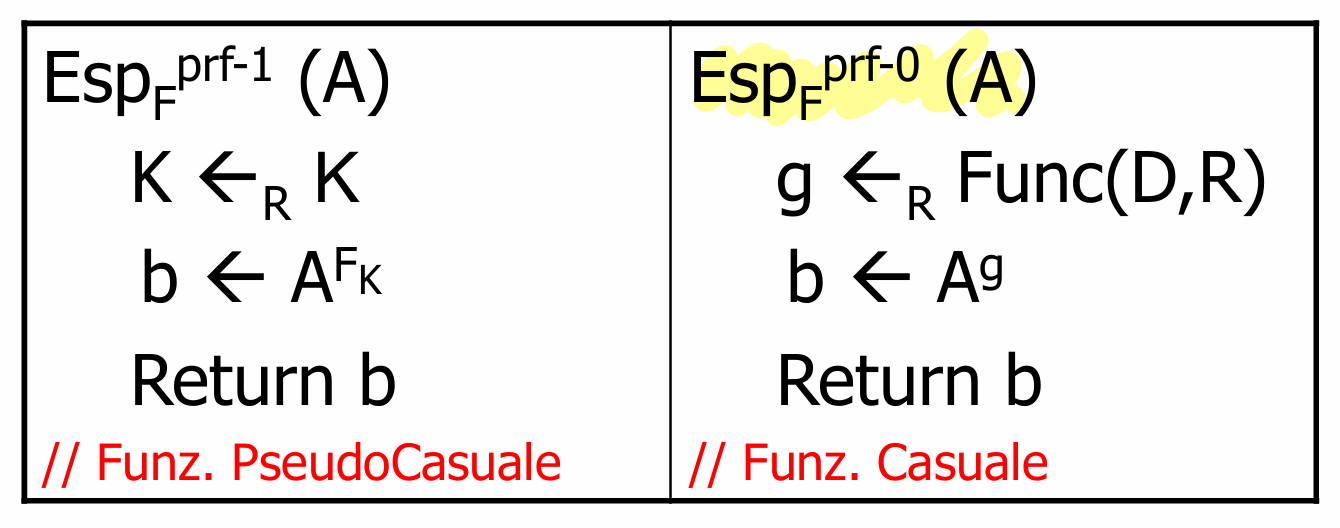
\includegraphics[width=0.8\linewidth]{Images/esperimento_random.png}
    \label{fig:esp_random}
\end{figure}

Definiremo vantaggio $Adv(A) = |Pr[Esp_F^{prf-1}(A)=1]-Pr[Esp_F^{prf-0}(A)=1]|$, più questo valore è piccolo, più la prf è sicura. 
Proviamo questa funzione 
\begin{figure}[H]
    \centering
    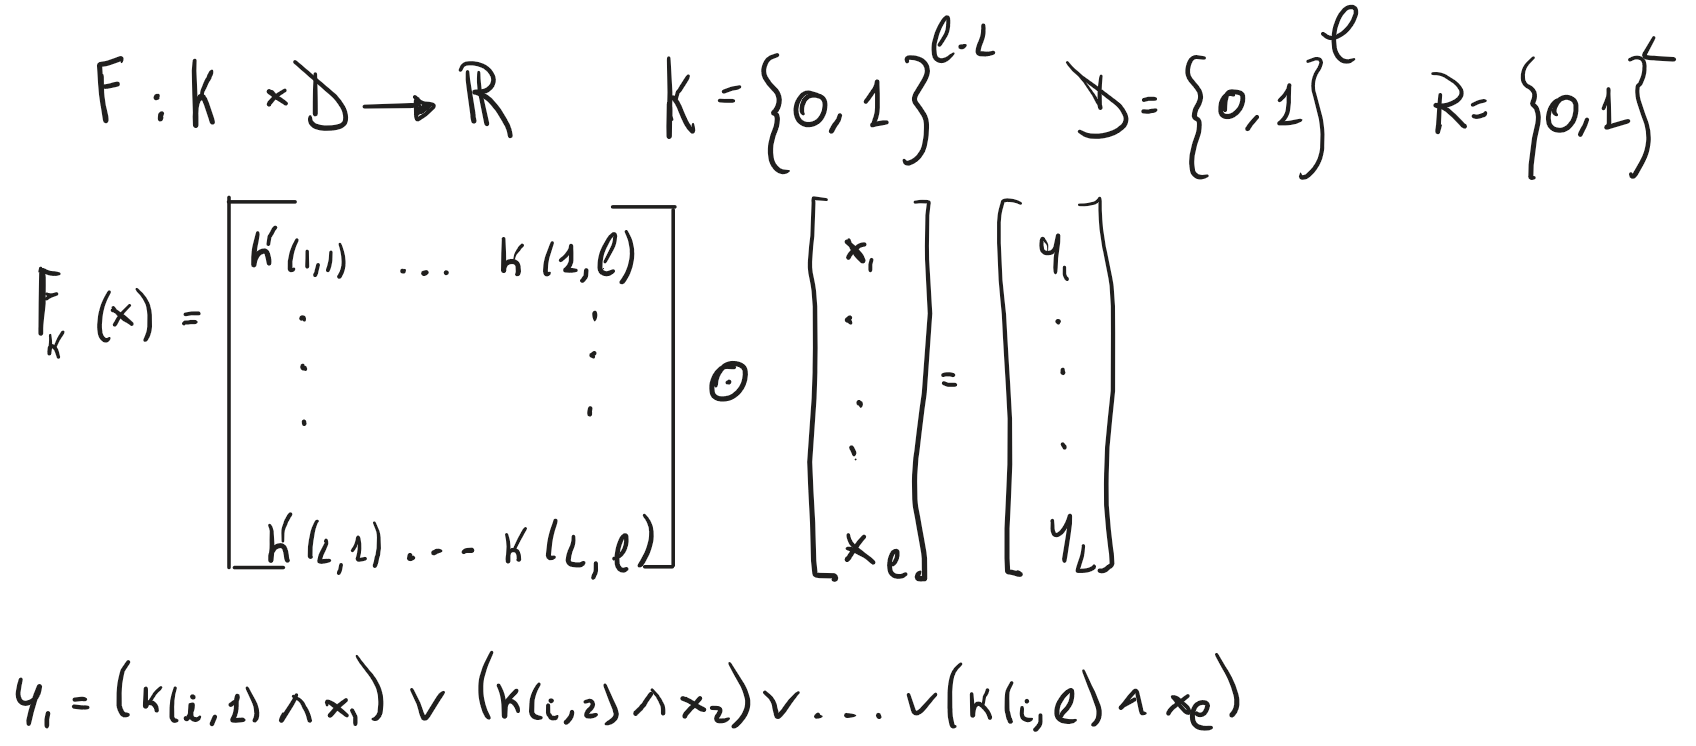
\includegraphics[width=1\linewidth]{Images/pseudo_random_esp.png}
\end{figure}
E testiamo con la definizione che abbiamo dato. Supponiamo di avere l'attaccante:
\begin{algorithm}[H]
\caption{Algoritmo $A(F)$}
\begin{algorithmic}[1]
    \State $x \gets 0^l$ \Comment{Stringa di $l$ zeri}
    \State $y \gets F(x)$ \Comment{Interroga l'oracolo $F$}
    \If{$y == 0^l$}
        \State \Return 1
    \Else
        \State \Return 0
    \EndIf
\end{algorithmic}
\end{algorithm}
Allora possiamo verificare le probabilità:
\begin{align*}
    &Pr[Exp^{prf-1}(A)=1]=1\quad Pr[Exp^{prf-0}(A)=1]=1/2^L
\end{align*}
Il vantaggio è $Adv(A) = 1-1/2^L$

Per continuare ad esercitarci, immaginiamo adesso di avere utilizzare una prf che è praticamente one-time-pad che però viene usata più volte e creiamo un attaccante.
\begin{algorithm}[H]
\caption{Algoritmo $A(F)$}
\begin{algorithmic}[1]
    \State $x_1 \gets 0^l$ \Comment{Stringa di $l$ zeri}
    \State $y_1 \gets F(x_1)$ \Comment{Ritorna la chiave k}
    \State $x_2 \gets y_1$ 
    \State $y_2 \gets F(x_2)$
    \If{$y_2 == 0^l$}\Comment{La chiave xor sé stessa fa $0^l$}
        \State \Return 1
    \Else
        \State \Return 0
    \EndIf
\end{algorithmic}
\end{algorithm}

Per cui, le probabilità sono $Pr[Exp^{prf-1}(A)=1]=1\quad Pr[Exp^{prf-0}(A)=1]=1/2^l$ e il vantaggio è $Adv(A) = 1-1/2^l$.
\\
\section{PRF implica sicurezza da Key Recovery}
Data questa definizione, abbiamo capito che effettivamente la proprietà di pseudo-randomicità è sintomo di sicurezza. Tuttavia il problema principale di ciò è che non possiamo dimostrare che un cifrario sia pseudo-casuale. Quello che faremo sarà assumere che il cifrario lo sia e, sulla base di ciò agiremo. L'idea è che legheremo la pseudo casualità ad un altro grande problema dell'informatica e faremo sì che se si riesce a rompere quello, allora si risolve il problema\footnote{Problema che non è mai stato risolto e, probabilmente, non lo sarà mai.}. \\
Supponiamo di voler dimostrare che la PRF implichi sicurezza da key recovery in maniera diretta. Prima di tutto facciamo sì che tutto sia ricondotto agli stessi termini così da poterne fare il confronto. Definiamo B, l'attaccante che si occuperà di attaccare il cifrario per Key recovery. 
\begin{figure}[H]
    \centering
    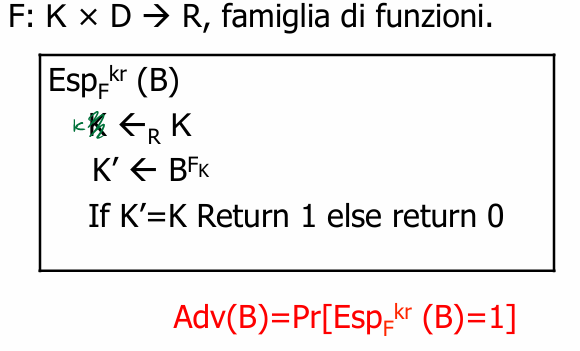
\includegraphics[width=0.5\linewidth]{Images/attacco_key_recovery.png}
\end{figure}
E, indicando con A l'attaccante che attacca il cifrario per indistinguibilità, vogliamo che 
\[Adv(B) \leq Adv(A)\]
Questa è molto interessante poiché notiamo come se l'attacco di key recovery funziona, allora l'attacco per indistinguibilità deve essere almeno buono tanto quello ma, se l'attacco per indistinguibilità è uguale a 0, allora lo sarà anche l'altro. 

Descriviamo l'attaccante A:
\begin{figure}[H]
    \centering
    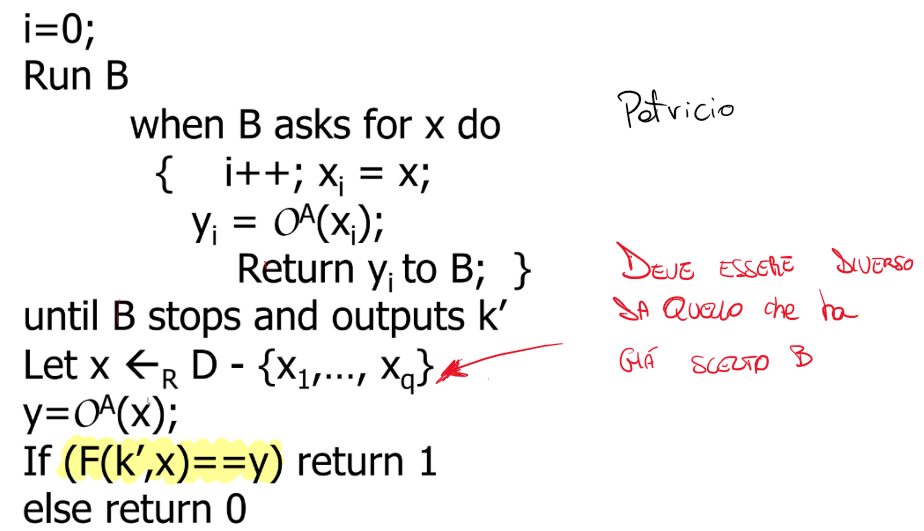
\includegraphics[width=0.6\linewidth]{Images/attaccante_indistinguibilita.png}
\end{figure}

Dimostriamo che quella relazione vale sempre.
\[Pr[Esp^{prf-1}(A)=1]\geq Adv(B)\]
 Può accedere se B è bravo e quindi io dico 1, o se B spara a caso e sbaglio e io, per puro caso, ho l'if vero. Invece:
 \[Pr[Esp^{prf-0}(A)=1]=\frac{1}{|R|}\]
 Da questo, segue che 
 \[Pr[Esp^{prf-1}(A)=1]-Pr[Esp^{prf-0}(A)=1]\geq Adv(B)-1/|R|\]

\section{Atacco del compleanno}
Supponiamo di avere $E:\{0,1\}^k \times \{0,1\}^n \xrightarrow{} \{0,1\}^n$ una famiglia di permutazioni. Supponiamo di ricevere un accesso black box ad una funzione casuale $g$ che è o un'istanza di E o una funzione casuale. 
Immaginiamo di voler distinguere i due casi, possiamo invocare la funzione su q punti e, se $g$ è una permutazione, ci basterà verificare che questa sia diversa per ogni punto. A primo impatto questo attacco sembra essere poco efficace, d'altro trovare tutte le possibili combinazioni non è fattibile. Tuttavia, vedremo che in realtà le probabilità sono molte più di quelle che possiamo immaginare grazie a quello che viene definito \textbf{paradosso del compleanno}. Di fatto, vedremo che basteranno più o meno $q = \sqrt{2^l}$ domande per avere un vantaggio prossimo a 1.

Il motivo per cui accade ciò è banalmente da imputare ad un dettaglio fondamentale della domanda. Noi non vogliamo trovare una specifica collisione, a noi ce ne basta una tra tutte le possibili coppie e non tra una specifica coppia. 

Supponiamo di avere $q$ palline e $N$ buche e, in base a ciò, supponiamo di voler valutare la probabilità che due palline finiscano nella stessa buca considerando che ogni pallina può finire in una qualsiasi delle buche con la stessa probabilità. Naturalmente se le buche sono meno delle palline per il teorema del Pigeon Hole questo sarà un evento certo, per cui, valutiamo il caso in cui $N >>> q$. Valutiamo gli eventi più sempici, sia $D_i$ l'evento che non vi sia alcuna collisione dopo aver lanciato l'iesima pallina.
\begin{align*}
    &Pr[D_1] = 1 \quad Pr[D_{i+1}|D_i] = \frac{N-1}{N}\\
    &\text{Proviamo a valutare $D_q$}\\
    &Pr[D_q] = Pr[D_q \land D_{q-1}]+Pr[D_q \land \! D_{q-1}]=\\
    &= Pr[D_q|D_{q-1}]Pr[D_{q-1}]+ Pr[D_q| \!D_q] Pr[!D_{q-1}]=\\
    &=Pr[D_q|D_{q-1}]Pr[D_{q-1}]=\\
    &= Pr[D_q|D_{q-1}]Pr[D_{q-1}|D_{q-2}]\dots Pr[D_2|D_{1}] Pr[D_1]=\\
    &=\prod_{i=1}^{q} (\frac{N-i}{N}) = \prod_{i=1}^{q} (1-\frac{i}{N}) \sim e^x  \quad x_i = i/N \quad 0< \frac{i}{N}<1\\
    &e^x = 1+x+\frac{x^2}{2!}+\frac{x^3}{3!}+\dots\\
    &e^{-x} = 1 - x+\frac{x^2}{2!}-\frac{x^3}{3!}\\
    &e^{-x} \sim 1-x  \\
    &\sim \prod_{i=1}^{q}e^{-\frac{1}{N}} = e^{-\sum_{i=1}^q \frac{i}{N}} = e^{-\frac{1}{N}\sum_{i=1}^{q}i} \sim e^{-\frac{q^2}{2N}}
\end{align*}  
Il nostro obiettivo è far sì che $Pr[!D_q] \geq 1/2$ per cui possiamo continuare così:
\begin{align*}
    &\frac{1}{2}=1-e^{-\frac{q^2}{2N}}\\
    &=\frac{1}{2} = e^{-\frac{q^2}{2N}}\\
    &= ln(\frac{1}{2})=-\frac{q^2}{2N} \xrightarrow{} q = \sqrt{2ln(2N)}
\end{align*}

Dunque, un cifrario a blocchi\footnote{I cifrari a blocchi sono considerati permutazioni perché, per una data chiave segreta, stabiliscono una corrispondenza biunivoca tra tutti i possibili blocchi di testo in chiaro e tutti i possibili blocchi di testo cifrato.} può essere distinto da una funzione casuale guardando un numero $2^{l/2}$ di coppie input-output.